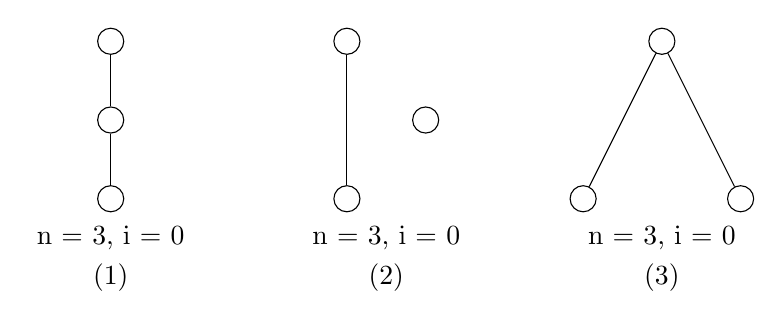
\begin{tikzpicture}
  \node[circle,draw=black] (A1) at (0, 0) {};
  \node[circle,draw=black] (A2) at (0, 1) {};
  \node[circle,draw=black] (A3) at (0, 2) {};

  \draw (A1) -- (A2) node {};
  \draw (A2) -- (A3) node {};
  \node (AL) at (0, -0.5) {n = 3, i = 0};
  \node (A) at (0, -1) {(1)};


  \node[circle,draw=black] (B1) at (3 + 0, 0) {};
  \node[circle,draw=black] (B2) at (3 + 0, 2) {};
  \node[circle,draw=black] (B3) at (3 + 1, 1) {};

  \draw (B1) -- (B2) node {};
  \node (BL) at (3 + 0.5, -0.5) {n = 3, i = 0};
  \node (B) at (3 + 0.5, -1) {(2)};


  \node[circle,draw=black] (C1) at (6 + 1, 2) {};
  \node[circle,draw=black] (C2) at (6 + 0, 0) {};
  \node[circle,draw=black] (C3) at (6 + 2, 0) {};

  \draw (C1) -- (C2) node {};
  \draw (C1) -- (C3) node {};
  \node (CL) at (6 + 1, -0.5) {n = 3, i = 0};
  \node (C) at (6 + 1, -1) {(3)};
\end{tikzpicture}